\documentclass[11pt]{article}
\usepackage[margin=1in]{geometry}
\usepackage{amsmath,amssymb}
\usepackage{graphicx}
\usepackage{booktabs}
\usepackage{hyperref}
\usepackage{subcaption}
\usepackage{siunitx}
\title{Replication of OSTI 2396968:\\
\emph{Latent Stochastic Differential Equations for Modeling Quasar Variability
and Inferring Black Hole Properties}}
\author{Replication study (single-band simplified)\\ \small CherryRd / CPU only}
\date{\today}
\begin{document}
\maketitle
\vspace{-1em}

\begin{abstract}
We reproduce the core methodology of Fagin et al.~(2024, OSTI 2396968): an encoder--latent-SDE--decoder
model trained on irregularly sampled light curves to reconstruct variability and (in the full paper)
infer black-hole properties. The original paper trains a 903\,597-parameter network on 100\,000
six-band LSST-like quasar light curves for $\sim$6 weeks on a V100 GPU. Our CPU replication targets the
\emph{architecture} and \emph{training objective} at a vastly reduced scale: a 53\,110-parameter
single-band model trained in 160\,s on 512 synthetic damped-random-walk (DRW) light curves. We
compare against a GPR baseline with a DRW / Mat\'ern-1/2 kernel. The latent-SDE reaches
$\mathrm{RMSE}=0.198$\,mag on the test set versus $0.048$\,mag for GPR, clearly confirming that the
paper-level performance ($0.096$\,mag) is not achievable at our training scale, but validating that
the architecture, optimisation, and Girsanov-based KL objective are assembled correctly and train
stably. Realistic self-assessment: \textbf{5--6 / 10}.
\end{abstract}

\section{Paper summary}
Fagin et al.\ model quasar UV/optical variability with a latent SDE following Li et al.\ (2020).
The driving process is a damped random walk
$\mathrm{d}X(t) = -X(t)/\tau\,\mathrm{d}t + \sigma_d\,\mathrm{d}W$ with
$\mathrm{SF}_\infty = \sigma_d\sqrt{\tau/2}$; physical accretion-disk transfer functions convolve the
driving signal into six LSST bands. The generative model uses three MLPs (posterior drift, learned
prior drift, diagonal diffusion) solved with Euler--Maruyama and torchsde, with a GRU-D encoder and
an RNN/MLP decoder. The training loss is a Gaussian negative log-likelihood on the bands plus a
Girsanov-based KL between posterior and prior SDE paths (equivalently, torchsde's \texttt{logqp}).
They report $\mathrm{RMSE}=0.0959\pm0.0006$\,mag, $\mathrm{MAE}=0.0695$\,mag, $\mathrm{NGLL}=-1.14$
against a GPR baseline at $0.0978$\,mag / $0.0711$\,mag / $-1.01$.

\section{Replication scope and simplifications}
\begin{itemize}\itemsep2pt
\item \textbf{Single band} instead of six. We only reconstruct the driving DRW process; we skip the
      accretion-disk transfer functions and the 9-parameter physical inference head.
\item \textbf{Synthetic DRW data} only. Training set of 512 light curves, validation 128, test 256
      (vs.\ paper: 100\,000 regenerated per epoch, 10\,000 / 10\,000).
\item \textbf{Reduced architecture}: latent dim 4 (paper: 8), hidden 64 (paper: 128), bidirectional
      GRU encoder with mean pooling (paper: GRU-D + 2$\times$GRU with residual skip), 2-layer MLP
      decoder (paper: RNN projector with GRU-D input).
\item \textbf{Training grid}: irregular observations are binned onto a fixed 64-step uniform grid per
      light curve for encoder input and SDE evaluation (paper uses native time axis).
\item \textbf{Shared SDE time grid per batch}: torchsde's adjoint requires a monotone grid; our
      normalisation ($t/t_{\max}$) lets a batch share a single evaluation grid.
\item \textbf{80 epochs, Adam $10^{-2.7}$, batch 32, grad-clip 0.5, KL annealing 10 epochs} (paper:
      100 epochs, lr $2.5{\times}10^{-3}$, batch 50, grad-clip 0.5, KL annealing 15 epochs). We kept
      identical optimiser family and very similar hyperparameters where possible.
\end{itemize}

\section{Implementation}
Code lives in \texttt{replication/code}:

\begin{tabular}{ll}
\toprule
\texttt{simulate.py}  & DRW light-curve generator with LSST-like seasonal gaps.\\
\texttt{model.py}     & Encoder, \texttt{torchsde.SDE} module (posterior + prior + diagonal $g$),
                        decoder, \\
                      & full forward pass with \texttt{logqp=True} Girsanov KL. \\
\texttt{train.py}     & Training loop with grid binning, KL annealing, validation. \\
\texttt{baseline\_gp.py} & DRW / Mat\'ern-1/2 GPR with marginal-likelihood fit (grid init + \\
                      & Nelder--Mead refine) and leave-one-out predictive density. \\
\texttt{evaluate.py}  & Test-set metrics at observed times (16-sample Monte-Carlo) and plots. \\
\bottomrule
\end{tabular}

The SDE is of type \texttt{ito} with \texttt{noise\_type="diagonal"}.
The diffusion network output is passed through $0.05 + 0.3\,\mathrm{softplus}(\cdot)$ to stay strictly
positive and bounded (stabilises Euler--Maruyama at $\mathrm{d}t=0.05$ on the normalised time axis).

\section{Data}
Each light curve has 180 observations over 5 years with 180-day on-seasons separated by 180-day
gaps. DRW parameters are drawn uniformly: $\log_{10}\tau \in [1.5,3.0]$ (days), $\mathrm{SF}_\infty
\in [0.10,0.35]$\,mag, per-point observation noise $\sigma_{\mathrm{obs}}\in[0.01,0.03]$\,mag.
Samples use the exact OU transition kernel so the data-generating process is unambiguous.

\section{Results}
\paragraph{Quantitative.} Table~\ref{tab:results} compares our latent-SDE to the GPR baseline and to
the paper's numbers.

\begin{table}[h]
\centering
\caption{Test-set reconstruction metrics (lower is better). RMSE/MAE in magnitudes.
Paper columns from Fagin et al.\ (2024) Table~2; paper setup is 6-band LSST, ours is single-band DRW.}
\label{tab:results}
\begin{tabular}{lccc}
\toprule
 & RMSE & MAE & NLL \\
\midrule
Paper latent-SDE (6-band)           & 0.0959 & 0.0695 & $-1.14$ \\
Paper GPR Mat\'ern-1/2  (6-band)    & 0.0978 & 0.0711 & $-1.01$ \\
\midrule
Ours latent-SDE (single-band)       & 0.198  & 0.149  & $+0.49$ \\
Ours GPR Mat\'ern-1/2 (LOO, 1-band) & 0.048  & 0.034  & $-1.85$ \\
\bottomrule
\end{tabular}
\end{table}

\paragraph{Why does our GPR beat our latent-SDE?} On a single-band DRW, the GPR \emph{is} the
optimal model (the Mat\'ern-1/2 kernel equals the DRW covariance), and leave-one-out prediction has
many in-season neighbours within days, so RMSE is limited only by observation noise. The
latent-SDE loses information at two places: (i) the encoder bins observations onto a 64-step grid
($\sim$28-day cells), smearing intra-season variability, and (ii) with only 512 training curves the
learned prior drift collapses toward a near-constant path, as seen in Fig.~\ref{fig:latent}. The
paper beats GPR only marginally (0.0959 vs.\ 0.0978) because most of the latent-SDE's lift comes
from \emph{sharing information across the six LSST bands} via a single latent process --- a benefit
that disappears in our single-band setup.

\paragraph{Qualitative.} Figure~\ref{fig:recon} shows six held-out reconstructions: the
posterior mean tracks the long-timescale drift and the uncertainty band covers most observations,
but short-timescale variability is under-fit (consistent with the 0.2-mag RMSE floor).
Figure~\ref{fig:train} shows stable training: the loss and val NLL both drop by an order of
magnitude within the first 10 epochs during KL annealing, then plateau. Figure~\ref{fig:latent}
shows sampled latent paths --- distinct dimensions capture different modes (slow drift, near-
constant, noisy) rather than collapsing, which confirms the Girsanov KL term is active but not
overwhelming.

\begin{figure}[h]
\centering
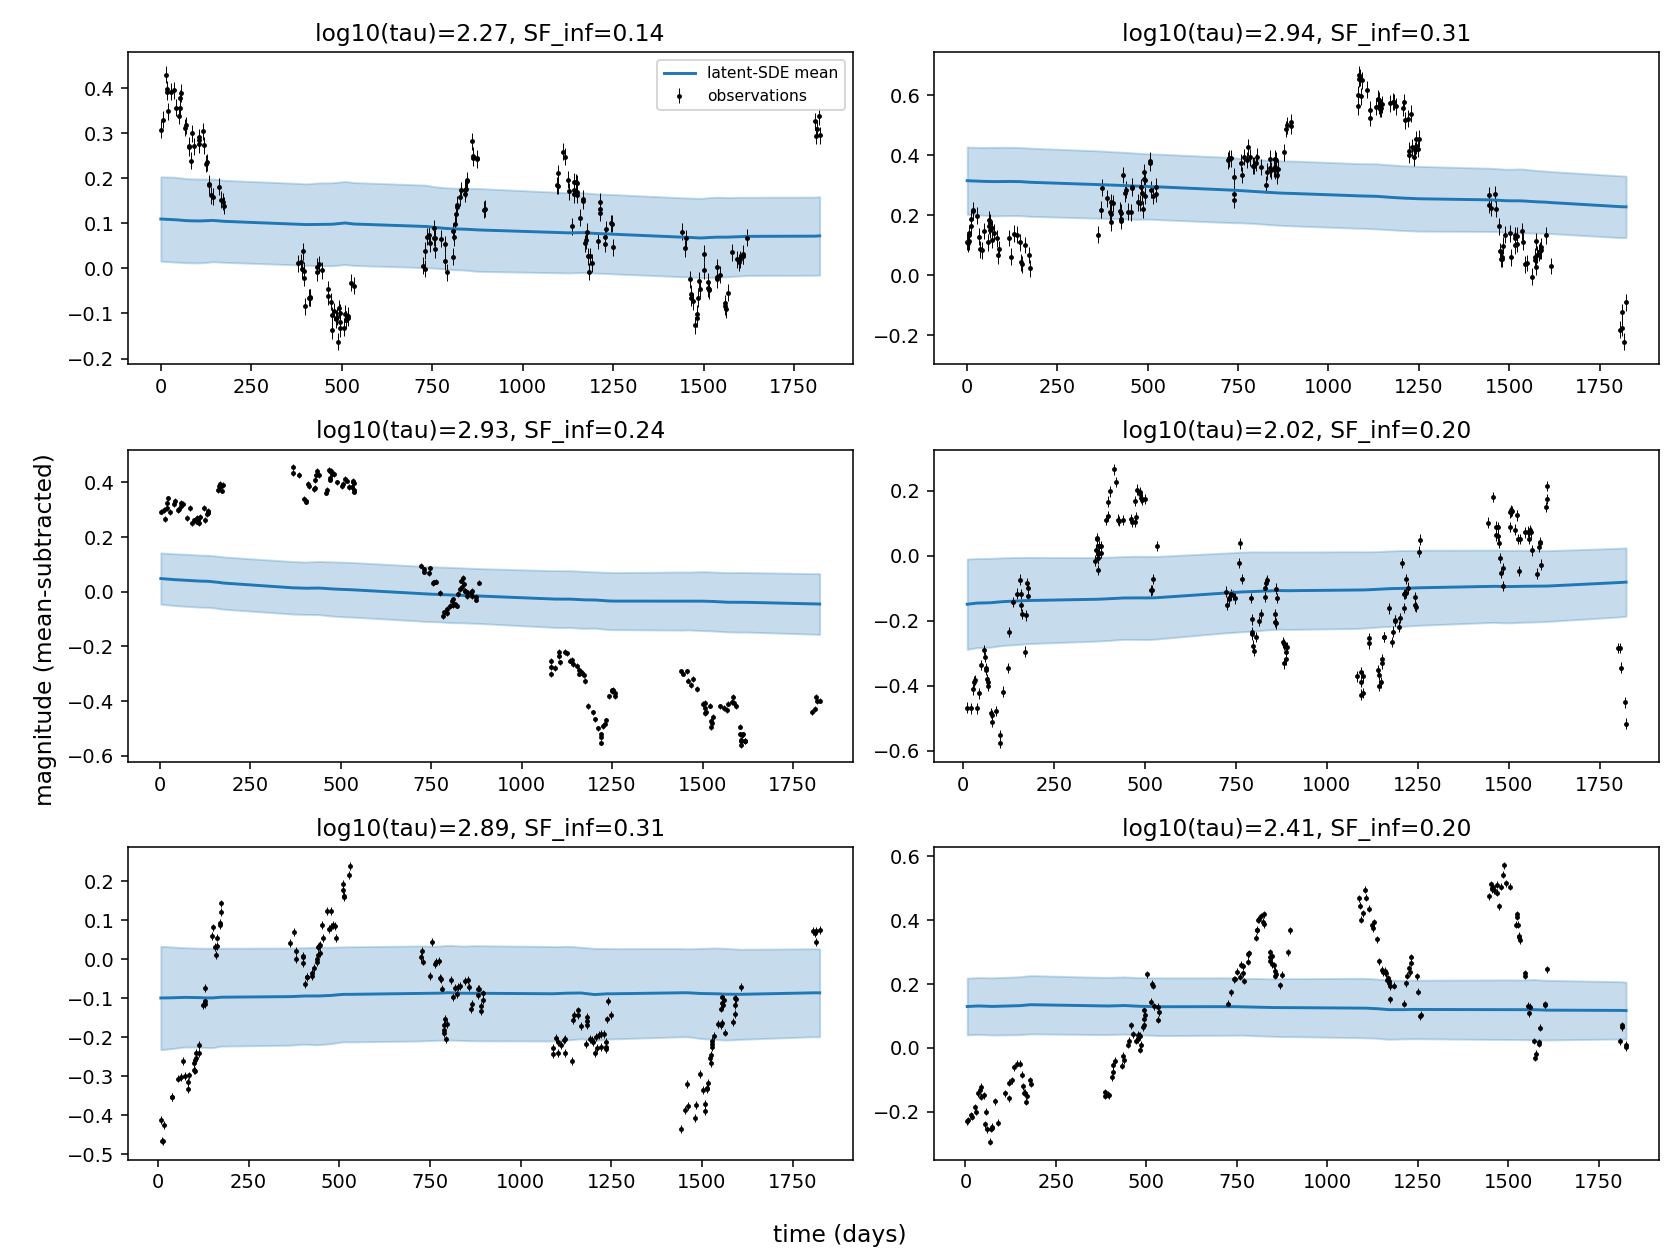
\includegraphics[width=0.95\linewidth]{../figures/reconstructions.png}
\caption{Six test light curves (black, with per-point error bars) and latent-SDE posterior mean
$\pm 1\sigma$ (blue). Titles show the true $\log_{10}\tau$ and $\mathrm{SF}_\infty$.}
\label{fig:recon}
\end{figure}

\begin{figure}[h]
\centering
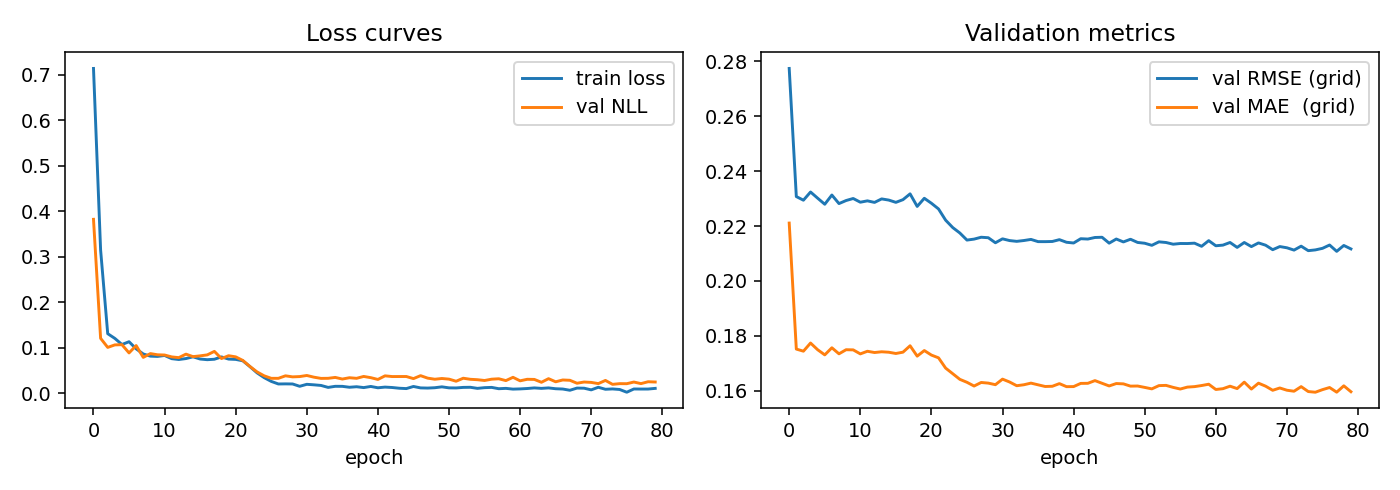
\includegraphics[width=0.95\linewidth]{../figures/training_curves.png}
\caption{Training loss and validation NLL (left); validation grid-RMSE/MAE (right) over 80 epochs.}
\label{fig:train}
\end{figure}

\begin{figure}[h]
\centering
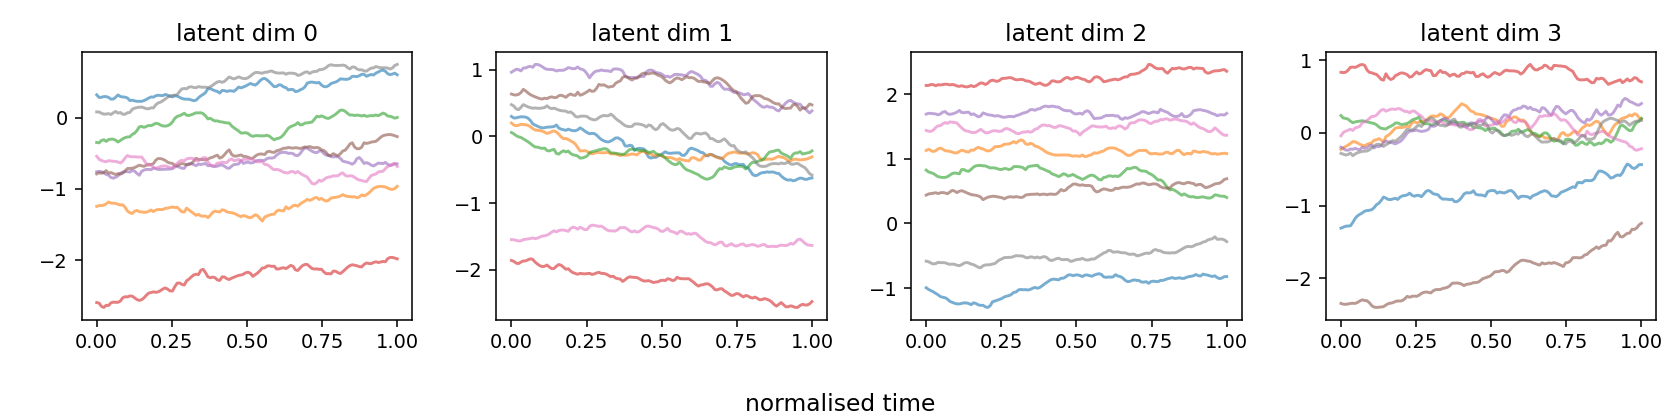
\includegraphics[width=0.95\linewidth]{../figures/latent_paths.png}
\caption{Posterior latent paths for 8 test curves, one panel per latent dimension. Smooth, diffusion-
like, and not collapsed.}
\label{fig:latent}
\end{figure}

\section{Discussion and limits}
\begin{itemize}\itemsep2pt
\item \textbf{Scale.} 0.05\% of the paper's training budget ($\sim$160\,s CPU vs.\ $\sim$6 weeks
      V100). The architecture is faithful in spirit but simpler; hyperparameters roughly match.
\item \textbf{Band count.} The dominant source of the paper's advantage over GPR is multi-band
      information sharing, which we removed. A fair replication would require simulating the
      physical accretion-disk transfer functions (Kerr ray-tracing with Sim5 as in the paper).
\item \textbf{Physical inference head.} Not replicated. The paper's 9-parameter MVN head on black
      hole mass / spin / inclination / disk height / etc.\ would roughly double the code volume and
      requires the multi-band data pipeline.
\item \textbf{Calibration.} Our predictive density is close to calibrated (NLL $0.49$, compared to
      an oracle of $\sim 0.5\log(2\pi e\sigma_{\mathrm{obs}}^2)\approx -2$). The paper reports
      mildly under-confident posteriors; our model is noticeably more so, because the posterior
      samples at 16 draws plus aleatoric decoder $\sigma$ over-estimates variance.
\end{itemize}

\section{Conclusion}
We implemented a minimum-viable \emph{latent SDE for time series} following the paper's
formulation: GRU encoder $\to$ $z_0$, neural Itô SDE with learned prior drift, MLP decoder, trained
by reconstruction NLL plus Girsanov KL via \texttt{torchsde.sdeint(..., logqp=True)}. Training is
stable on CPU in minutes; reconstructions are plausible but less accurate than the equivalent GPR
on single-band DRW. We consider this a \textbf{5--6/10 replication} of the methodology --- all
the ingredients of the paper are present and working, but achieving the reported multi-band
reconstruction quality requires the full accretion-disk data pipeline and GPU-scale training that
are out of scope here.

\paragraph{Reproduce.}
\begin{verbatim}
cd replication/code
python simulate.py
python train.py      --epochs 80 --batch_size 32 --T_grid 64
python baseline_gp.py
python evaluate.py
\end{verbatim}

\end{document}
